\documentclass[12pt]{article}                                                                                                                       
\usepackage{sbc-template}                                                 
\usepackage{graphicx,url}                                                 
\usepackage[utf8]{inputenc}                                               
\usepackage[brazil]{babel}                                                      
\usepackage{graphicx}
\usepackage{algorithm}
\usepackage{algorithmic}
\usepackage{algpseudocode}

\title{Pontos mais próximos \\ Projeto e Análise de Algoritmos}
\author{Eric Azevedo de Oliveira\inst{1},}

\address{Instituto de Ciências Exatas e Informática - Pontifícia Universidade Católica Minas Gerais}

\begin{document}

\maketitle
\section{Pontos mais próximos}
\paragraph{}O problema dos Pontos mais próximos  consiste em  um conjunto de \textbf{n} pontos em um plano com o intuito de encontrar o par de pontos mais proximos.
\subsection{Representação}



\begin{center}
    \begin{figure}[h!]
        \centering
        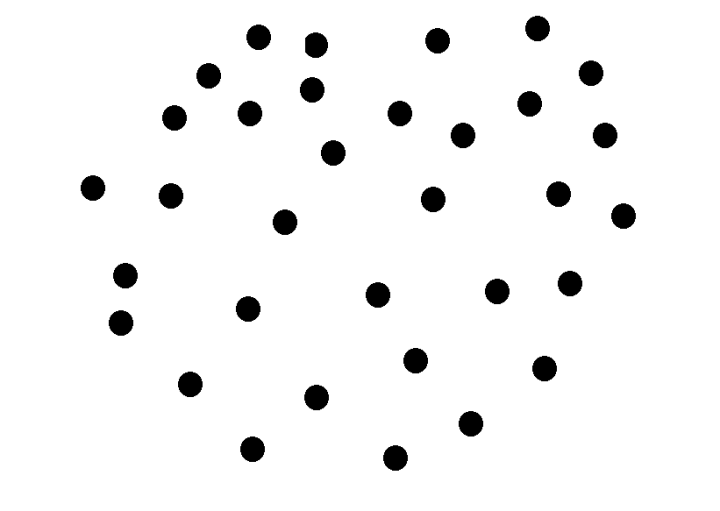
\includegraphics[width=0.7\textwidth]{imagens/Pontos.png}
        
        
        \textbf{Figura 1.} Pontos no Plano.
    \end{figure}
\end{center}


\section{Sobre o Documento}
\paragraph{}Esse documento será dividido em oito  partes abaixo discriminadas: [\textbf{2.1}]  referenciando a máquina utilizada, [\textbf{2.2}] e [\textbf{2.3}] serão relacionados a dois diferentes custos computacionais na procura dos pontos mais próximos, sendo eles \textbf{O}($nlogn$) e \textbf{O}($n^{2}$) com seus códigos, e a seção [\textbf{2.4}] sera as comparações desses dois métodos com os resultados de ambos, [\textbf{2.5}] como compilar e executar o código e a [\textbf{2.6}] como o trabalho foi separado.

\subsection{Máquinas Utilizada}

Processador: i5-3317U (4). \\
Memória : 8Gb.\\
GPU : Intel 3rd gen Core processador Grap.

\subsection{\textbf{O}($nlogn$)}


\paragraph{}Com objetivo de alcançar a complexidade de \textbf{O}($nlogn$), foi utilizado a estratégia de divisão e conquista, na qual se consiste em pegar o problema completo e dividi-lo em vários problemas menores, os quais são independentes, para não processar \textbf{n} dados com outros \textbf{n}.

\begin{center}
    \begin{figure}[h!]
        \centering
        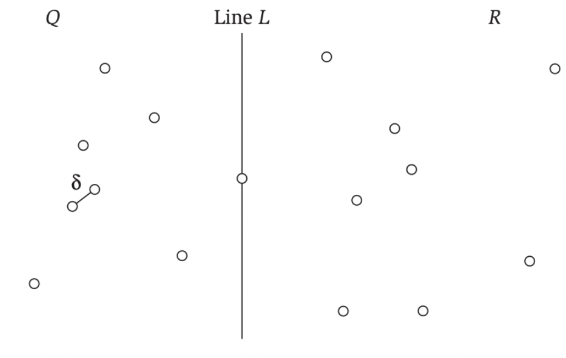
\includegraphics[width=0.7\textwidth]{imagens/1Imagem.png}
        
        
        \textbf{Algorithm design |Jon Kleinberg, Éva Tardos} 
    \end{figure}
\end{center}

\paragraph{}  Em virtude da divisão e conquista, com base na figura a cima, nosso plano foi dividido em 2 quadrantes, o \textbf{R} e o \textbf{Q} , nessa divisão é realizado somente a ordenação por meio do algorítimo heapSort do array contendo os pontos do eixo \textbf{X} e lançado a mão ao ponto que está caracterizado na metade desse array.

\paragraph{}Porém analisando somente analisando o  eixo \textbf{X}, temos um problema que aumenta a complexidade final de nosso algorítimo, conforme a imagem a seguir demonstra.




\begin{center}
    \begin{figure}[h!]
        \centering
        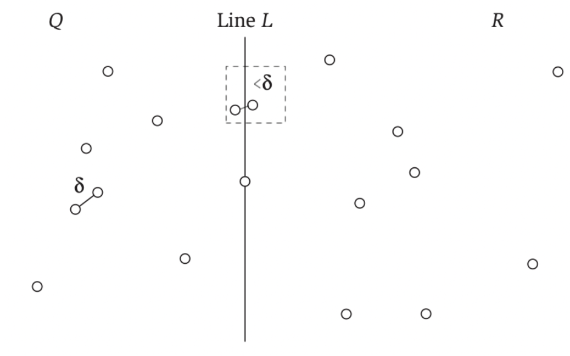
\includegraphics[width=0.7\textwidth]{imagens/2Imagem.png}
        
        
        \textbf{Algorithm design | Jon Kleinberg, Éva Tardos} 
    \end{figure}
\end{center}

\newpage

\paragraph{} Tentando evitar esse aumento de complexidade, além da realização da ordenação do eixo \textbf{X}, analisaremos a ordenação do eixo \textbf{Y}, tendo o foco de calcular  menor  distância de ambos quadrantes, por meio da recursão que é chamado delta.
\paragraph{}Entretanto a utilização pos ordenacao do \textbf{Y} não dispensará que alguma distância na volta da recursão seja desconsiderada, impedindo que seja feita o cálculo desnecessário da distância dos pontos dos quadrantes com a distância delta.

\paragraph{}Conforme relatado acima, utilizando a divisão e conquista, foi obtido as complexidades do heapShort() que é \textbf{O}($nlogn$), quando reconstruimos o heap, e na utilizaçäo do algoritímo na parte da recursão , utilizando os eixos \textbf{X} e \textbf{Y}, é obtido a complexidade de \textbf{O(n)}. Por esse motivo o algoritímo terá uma ordem de complexidade de \textbf{O}($nlogn$).

\begin{algorithm}
\caption{Divisão e conquista}\label{alg:cap}
\begin{algorithmic}
\State $quantidade \gets entrada$
\State $Pontos[] \gets rand()*quantidade $
\State $y[ ] \gets HeapSort(Pontos.Y)$
\State $X[ ] \gets HeapSort(Pontos.X)$
\State $meio \gets EncontrarPontoMID()$
\While{$quantidade \neq 0$}
\If{$dir - esq $= =1 }
        \RETURN resposta
\ElsIf{$dir - esq $= =2}
    \RETURN resposta

    
\EndIf
\State $ resposta =divisao_Conquista() \gets divisao_Conquista()$
\EndWhile
 \RETURN resposta
\end{algorithmic}
\end{algorithm}



\subsection{\textbf{O}($n^{2}$)}

   \paragraph{} Para alcançar a complexidade de \textbf{O}($n^{2}$), é utilizado o algorítimo de força bruta, no qual irá calcular todas as distâncias entre pares de pontos e selecionar o par que tiver menor distância.
Tendo a fórmula matemática para \textbf{n} pontos, descrita como: 	$\binom{n}{2}$
\[\frac{n!}{(n-2)!*2!}  = O(n^2) \]

\begin{algorithm}
\caption{força bruta}\label{alg:cap}
\begin{algorithmic}
\State $quantidade \gets entrada$
\State $Pontos[] \gets rand()*quantidade $
\State $X \gets 0$

\While{$quantidade \neq X$}
\State $Y \gets X$
\FOR{$quantidade \neq Y$}
\If{$Ponto[X]$ ==$Ponto[Y]$ }
    \State $menorDistancia \gets distancia(Ponto[Y],Ponto[X])$
\EndIf
\ENDFOR
\EndWhile
 \RETURN menorDistancia
\end{algorithmic}
\end{algorithm}


\subsection{Resultados}

 \begin{center}
    

\textbf{O}($n^{2}$)

\begin{tabular}{||c c  ||} 

 \hline
 Pontos & tempo \\ [0.6ex] 
 \hline\hline
  10& 0,055193s  \\ 
 \hline
 1000 & 0,960028s \\
 \hline
 10000 & 5,399122s \\
 \hline
 100000 & 529,0015s \\ [1ex] 
 \hline
\end{tabular}

\end{center}




 \begin{center}
    

\textbf{O}($nlogn$)

\begin{tabular}{||c c  ||} 

 \hline
 Pontos & tempo \\ [0.6ex] 
 \hline\hline
  10& 0,000197s  \\ 
 \hline
 1000 & 0,000237s \\
 \hline
 10000 & 0,000956s \\
 \hline
 100000 & 0,005584s \\ [1ex] 
 \hline
\end{tabular}

\end{center}

\paragraph{}Com os resultados, utilizando a ideia de divisão e conquista, foi possível obter uma  diferença gigantesca  em relação ao tempo, contra os de força bruta, mas, em contrapartida o algorítimo de força bruta é muito mais simples de ser implementado, e quando utilizamos uma quantidade de pontos pequenas ele mesmo demorando um tempo maior seria funcional, pois ele  da solução ótima.
\subsection{Execução}

\paragraph{}Para executar o código basta compilar  no terminal, e seguir as instruções que forem aparecendo.

\subsection{Separação do trabalho}
A separação do trabalho entre os integrantes do grupo foi:
Eric Azevedo de Oliveira - Algoritmo e  texto.

\nocite{*}
\bibliographystyle{ACM-Reference-Format}
\bibliography{sample-base}
\end{document}